%%---------------------------------------------------------------------------%%
%% draco-5_0_0.tex
%% Thomas M. Evans
%% $Id$
%%---------------------------------------------------------------------------%%
\documentclass[note]{ResearchNote}
\usepackage[centertags]{amsmath}
\usepackage{amssymb,amsthm,graphicx}
\usepackage[mathcal]{euscript}
\usepackage{tabularx}
\usepackage{cite}
\usepackage{c++}
\usepackage{tmadd,tmath}
\usepackage{listings}
\usepackage{color}

%%---------------------------------------------------------------------------%%
%% DEFINE SPECIFIC ENVIRONMENTS HERE
%%---------------------------------------------------------------------------%%
%\newcommand{\elfit}{\ensuremath{\operatorname{Im}(-1/\epsilon(\vq,\omega)}}
%\msection{}-->section commands
%\tradem{}  -->add TM subscript to entry
%\ucatm{}   -->add trademark footnote about entry

\newcommand{\draco}{Draco}
\newcommand{\dracor}{\draco-5\_0\_0}
\newcolumntype{L}{>{\ttfamily}X}

\newcommand{\autoconf}{\textsf{Autoconf}}
\newcommand{\automake}{\textsf{Automake}} 
\newcommand{\CVS}{\textsf{CVS}}  
\newcommand{\make}{\textsf{Make}}

\newcommand{\tableText}[1]{{\raggedright #1}}


\definecolor{listingBG}{rgb}{0.95,0.95,0.95}

\lstset{language=csh,
  showstringspaces=false,
  frame=shadowbox,
  basicstyle=\footnotesize,
  rulesepcolor=\color{black},
  backgroundcolor=\color{listingBG}
}

%%---------------------------------------------------------------------------%%
%% BEGIN DOCUMENT
%%---------------------------------------------------------------------------%%
\begin{document}

%%---------------------------------------------------------------------------%%
%% OPTIONS FOR NOTE
%%---------------------------------------------------------------------------%%

\toms{Distribution}
%\toms{Joe Sixpak/XTM, MS B226}
\refno{CCS-4:04-XX (U)}
\subject{Release of \dracor}

%-------NO CHANGES
\divisionname{Computer and Computational Division}
\groupname{CCS-4:Transport Methods Group}
\fromms{Thomas M. Evans/CCS-4 D409\\
  Mike Buksas/CCS-4 D409\\
  Kelly Thompson/CCS-4 D409}    %
\phone{(505)665--3677}
\originator{tme}
\typist{tme}
\date{\today}
%-------NO CHANGES

%-------OPTIONS
%\reference{NPB Star Reimbursable Project}
%\thru{P. D. Soran, XTM, MS B226}
%\enc{list}      
%\attachments{list}
%\cy{list}
%\encas
%\attachmentas
%\attachmentsas 
%-------OPTIONS

\revisionnum{1}

%%---------------------------------------------------------------------------%%
%% DISTRIBUTION LIST
%%---------------------------------------------------------------------------%%

\distribution {

  CCS-4  MS D409:\\ 
  CCS-2  MS D413:\\ 
  Baker, Randal,     CCS-4  MS D409\\ 
  Budge, Kent,       CCS-4  MS D409\\ 
  Buksas, Michael,   CCS-4  MS D409\\ 
  Carrington, David, CCS-4  MS D409\\ 
  Dahl, Jon,         CCS-4  MS D409\\ 
  Densmore, Jeffery, CCS-4  MS D409\\ 
  Evans, Thomas,     CCS-4  MS D409\\ 
  Hungerford, Aimee, CCS-4  MS D409\\ 
  Olson, Gordon,     CCS-4  MS D409\\ 
  Thompson, Kelly,   CCS-4  MS D409\\ 
  Turner, Scott,     CCS-4  MS D409\\ 
  Urbatsch, Todd,    CCS-4  MS D409\\ 
  Ward, Robert,      CCS-4  MS B296\\ 
  Warsa, James,      CCS-4  MS D409\\ 
  Dilts, Gary,       CCS-2  MS D413\\ 
  Lowrie, Robert,    CCS-2  MS D413\\ 
  Morel, Jim,        CCS-2  MS D413\\ 
  Turner, John,      CCS-2  MS D413\\ 
  
}

%%---------------------------------------------------------------------------%%
%% BEGIN NOTE
%%---------------------------------------------------------------------------%%

\opening

\begin{abstract}
  
  We have released \dracor.  This release marks significant changes to
  \draco.  First and foremost, the \textsc{imc} and \textsc{mc}
  packages have been moved to the ClubIMC library.  Additional changes
  have been made to the \draco\ directory organization, build system,
  and automatic documentation system.

\end{abstract}

%%---------------------------------------------------------------------------%%

\section{\draco\ Contributors}

The following people are contributors to \draco:
\begin{center}
  \small
  \begin{tabular}{ll}
    Tom Evans & \texttt{tme@lanl.gov} \\
    Kelly Thompson & \texttt{kellyt@lanl.gov} \\
    Todd Urbatsch & \texttt{tmonster@lanl.gov} \\
    Kent Budge & \texttt{kgbudge@lanl.gov} \\
    Mike Buksas & \texttt{mwbuksas@lanl.gov} \\
    Jim Warsa & \texttt{warsa@lanl.gov} \\
    Rob Lowrie & \texttt{lowrie@lanl.gov} \\
    Todd Adams & \texttt{bta@lanl.gov} \\
    Paul Batcho & \texttt{batcho@lanl.gov} \\
  \end{tabular}
\end{center}

%%---------------------------------------------------------------------------%%

\section{\draco\ Component Packages}

\dracor\ contains the following component packages:
\begin{center}
  \footnotesize
  \begin{tabular}{lp{3.0in}}
    \hline\hline 

    c4 & \tableText{communication library} \\
    cdi & \tableText{Common Data Interface (CDI) component} \\
    cdi\_analytic & \tableText{CDI analytic data component} \\
    cdi\_gandolf & \tableText{CDI GANDOLF wrapper} \\
    ds++ & \tableText{data structures library} \\
    lapack\_wrap & \tableText{wrapper to BLAS and LAPACK} \\
    meshReaders & \tableText{mesh reader interface} \\
    meshReaders\_Services & \tableText{services for mesh readers
      (connectivity, etc)} \\ 
    pcgWrap & \tableText{wrapper for PCGLIB} \\
    plot2D & \tableText{2-D plotter interface built on XMGRACE} \\
    quadrature & \tableText{quadrature component} \\
    rng & \tableText{random number generators and SPRNG wrappers} \\
    RTT\_Format\_Reader & \tableText{\texttt{meshReaders}
      implementation for RTT format meshes} \\
    stdheaders & \tableText{C-standard libraries wrapped in the
      \texttt{std::} namespace} \\ 
    timestep & \tableText{a timestep controller component} \\
    traits & \tableText{traits used by other \draco\ components} \\
    units & \tableText{a physics units component} \\
    viz & \tableText{interfaces to visualization tools (EnSight)} \\
    xm & \tableText{glommable expression templates} \\  

    \hline\hline 
  \end{tabular}
\end{center}

The following table summarizes changes to \draco\ components since
\draco-4\_0\_0. 
\begin{center}
  \begin{tabular}{lp{4.0in}}
    \hline\hline 

    mc & \tableText{removed from \draco} \\
    imc & \tableText{removed from \draco} \\
    cdi\_eospac & \tableText{not included as part of \dracor\ because
      of EOSPAC/FORTRAN compiler issues; will be re-integrated when
      EOSPAC 6.0 is released} \\
    ds++ & \tableText{added reference counted field class
      (\texttt{RCF}) and a light-weight vector
      (\texttt{Vector\_Lite})} \\ 
    Draco Build System & \tableText{autodoc generation enhanced; MPI
      defaults on LINUX removed; added middleware vendor option for
      clients of the build system; see \S~\ref{sec:dbs} for details} \\
    tools & \tableText{added several new tools including
      \texttt{check\_for\_tags.py}, \texttt{numdiff.py},
      \texttt{update\_release\_tags.py}, and \texttt{profiler.py};
      updated \texttt{launchtest} script to work for IBM and use a
      cleaner implementation} \\
    \hline\hline 
  \end{tabular}
\end{center}

There are no inter/intra-component cyclic dependencies in \draco.  The
levelized graph for \dracor\ components is shown in
Fig.~\ref{fig:level}.
\begin{figure}
  \label{fig:level}
  \centerline{
    \includegraphics[height=5.5in]{level-5_0_0.ps}}
  \caption{\dracor\ levelized component graph.  Dotted lines signify
    that the dependency if only required for testing.}
\end{figure}

Lines-of-Code (LOC) statistics for the last four \draco\ releases are
are shown in Fig.~\ref{fig:stats}.  The large drop between
\draco-4\_0\_0 and \dracor\ is due to the removal of the \textsc{mc}
and \textsc{imc} packages. The aggregate LOC statistics for \dracor\ 
are:
\begin{center}
  \begin{tabular}{|l|l|} \hline
    Total component package source code & 8363 \\
    Total unit test code & 12479 \\
    Total DBC statements & 680 \\
    Total comments & 20891 \\
    \hline
  \end{tabular}
\end{center}
\begin{figure}
  \label{fig:stats}
  \centerline{
    \includegraphics[width=6in]{loc-5_0_0.eps}}
  \caption{LOC statistics for \dracor\ component packages.}
\end{figure}
Table~\ref{tab:loc} shows LOC metrics for each \draco\ component in
\dracor.  LOC metrics are stored in \draco\ in
\texttt{draco/doc/code\_stats}.
\begin{table}
  \caption{
    LOC metrics for component packages in \dracor.  DBC LOC refers to
    Design-by-Contract$^{\copyright}$ statements. 
  }
  \label{tab:loc}
  \begin{center}
    \begin{tabular}{llll}\hline\hline
      \multicolumn{1}{c}{Component} &
      \multicolumn{1}{c}{Source LOC} &
      \multicolumn{1}{c}{DBC LOC} &
      \multicolumn{1}{c}{Test LOC} \\\hline
      
      c4        &       582     &       19      &       407     \\
      cdi       &       371     &       60      &       772     \\
      cdi\_analytic      &       516     &       120     &       493     \\
      cdi\_gandolf       &       665     &       25      &       713     \\
      ds++      &       1680    &       190     &       5769    \\
      lapack\_wrap       &       77      &       37      &       116     \\
      meshReaders       &       657     &       33      &       831     \\
      meshReaders\_Services      &       265     &       9       & 269 \\
      pcgWrap   &       224     &       9       &       79      \\
      plot2D    &       227     &       20      &       75      \\
      quadrature        &       560     &       48      &       64      \\
      rng       &       115     &       15      &       158     \\
      RTT\_Format\_Reader &       1265    &       38      &       1041    \\
      stdheaders        &       4       &       0       &       0       \\
      timestep  &       335     &       16      &       127     \\
      traits    &       87      &       9       &       49      \\
      units     &       215     &       8       &       1185    \\
      viz       &       361     &       20      &       74      \\
      xm        &       157     &       4       &       257     \\
      \hline\hline
    \end{tabular}
  \end{center}
\end{table}

With the adoption of the \textsf{Bullseye} coverage analysis tool, we
are better able to track unit-test coverage of \draco\ components.
The goal is to achieve 100\% functional test coverage for each \draco\
component.  Table~\ref{tab:coverage} gives functional and conditional
point coverage for \dracor.
%%---------------------------------------------------------------------------%%
%% coverage table for draco-5_0_0
%%---------------------------------------------------------------------------%%


\begin{table}
  \caption{
    Unit-test coverage in \dracor.  C/D Coverage refers to conditional
    statements.  We strive for 100\% function point coverage.  
  }
  \label{tab:coverage}
  \begin{center}
    \begin{tabular}{lllll}\hline\hline
      \multicolumn{1}{c}{Component} &
      \multicolumn{1}{c}{Function Coverage} &
      \multicolumn{1}{c}{Percent (\%)} &
      \multicolumn{1}{c}{C/D Coverage} &
      \multicolumn{1}{c}{Percent (\%)} \\\hline
      pcgWrap       &       16      /       31      &       51.00   &       24      /       55      &       43.00   \\
      xm     &       89      /       169     &       52.00   &       29      /       32      &       90.00   \\
      c4     &       56      /       102     &       54.00   &       14      /       40      &       35.00   \\
      ds++   &       318     /       511     &       62.00   &       227     /       542     &       41.00   \\
      cdi\_gandolf    &       63      /       101     &       62.00   &       93      /       172     &       54.00   \\
      lapack\_wrap    &       11      /       17      &       64.00   &       0       /       0       &       0       \\
      traits &       12      /       17      &       70.00   &       0       /       0       &       0       \\
      plot2D &       20      /       28      &       71.00   &       50      /       84      &       59.00   \\
      quadrature     &       28      /       38      &       73.00   &       75      /       123     &       60.00   \\
      timestep      &       49      /       62      &       79.00   &       85      /       178     &       47.00   \\
      meshReaders\_Services   &       17      /       21      &       80.00   &       114     /       136     &       83.00   \\
      rng    &       20      /       24      &       83.00   &       12      /       18      &       66.00   \\
      cdi\_analytic   &       66      /       76      &       86.00   &       66      /       82      &       80.00   \\
      cdi    &       26      /       29      &       89.00   &       46      /       64      &       71.00   \\
      viz    &       9       /       10      &       90.00   &       103     /       142     &       72.00   \\
      meshReaders    &       32      /       34      &       94.00   &       236     /       386     &       61.00   \\
      RTT\_Format\_Reader      &       309     /       319     &       96.00   &       392     /       563     &       69.00   \\
      units  &       83      /       83      &       100.00  &       58      /       58      &       100.00  \\
      \hline
      {\bf Total} & {\bf 1249/1746} & {\bf 71.53} & {\bf 1657/2719} &
      {\bf 60.94} \\

      \hline\hline
    \end{tabular}
  \end{center}
\end{table}

%%---------------------------------------------------------------------------%%
%% end of coverage table
%%---------------------------------------------------------------------------%%


%%---------------------------------------------------------------------------%%

\section{\draco\ Build System}
\label{sec:dbs}

The \draco\ Build System (DBS) has undergone some significant
changes.  The most significant updates are in the automatic
documentation system.  The auto-documentation system can now be
seamlessly imported into client code-systems.  This is a new feature.
A full description of the auto-documentation system is available in
\cite{ccs-4:04-35}. 

A brief list of other changes to the DBS is:
\begin{itemize}
\item LINUX defaults for the MPI vendor have been removed; it is now
  necessary to add \texttt{--with-mpi-inc} and \texttt{--with-mpi-lib}
  at compile time
\item the DBS can now be used in ``middleware'' component libraries
\item most scripting in the makefiles is now gone; the functionality
  is now performed in the configure scripts
\item general cleanup and organizational fixes
\end{itemize}

%%---------------------------------------------------------------------------%%

\section{\draco\ Directory Structure}

As part of project Thuban~\cite{ccs-4:04-21} we have done some
substantial reorganization of the \draco\ directory structure.  This
reorganization was done to make exporting the \draco\ development
environment easier.  The new \draco\ directory structure is shown below: 
\begin{lstlisting}[basicstyle=\footnotesize, xleftmargin=2.0in, 
  xrightmargin=2.0in]
draco/
    src/
        ds++/
        c4/
        ...
    doc/
        gettingStarted/
        releases/
        ...
    tools/
    autodoc/
    config/
    environment/
        elisp/
        templates/
        bibfiles/
        bibtex/
        latex/
\end{lstlisting}
The \texttt{environement/} directory is where all of the changes have
been made.  Table~\ref{tab:envdir} describes these changes in detail.
The rest of the \draco\ directory structure remains unaltered,
although the contents of the directories may have changed.
\begin{table}
  \caption{
    Descriptions of the directories in \texttt{draco/environment}.
    The \draco\ development environment is entirely encapsulated
    within the \texttt{environment} directory.
  }
  \label{tab:envdir}
  \begin{center}
    \begin{tabular}{lp{3in}}\hline\hline
      \multicolumn{1}{c}{Directory} & 
      \multicolumn{1}{c}{Description} \\ \hline
      
      \texttt{elisp} & \tableText{the \draco\ XEmacs macro
        definitions; this directory formerly sat in
        \texttt{draco/elisp}} \\ 
      
      \texttt{templates} & \tableText{code, build system, and
        documentation templates; this directory formerly sat in
        \texttt{draco/templates}} \\

      \texttt{bibfiles} & \tableText{bibliography databases
        (\texttt{.bib} files); the contents of this directory have
        been ported from \texttt{draco/doc/bib} and other places} \\ 
      
      \texttt{bibtex} & \tableText{bibliography style files
        (\texttt{.bst} files); this directory formerly sat in
        \texttt{archive/tex} (in the CCS-4 CVS repository)} \\
      
      \texttt{latex} & \tableText{latex class and style files
        (\texttt{.cls} and \texttt{.sty} files); this directory
        formerly sat in \texttt{archive/tex} (in the CCS-4 CVS
        repository)} \\ 

      \hline\hline
    \end{tabular}
  \end{center}
\end{table}

The reason for this change was to make exporting the \draco\
development environment easier.  Clients can simply import
\texttt{environment} into their source development trees and take
advantage of \draco's powerful XEmacs and \LaTeX\ tools. 

The \draco\ Build System (DBS), encapsulated within
\texttt{draco/config}, is separate from the \draco\ development
environment sitting in \texttt{environment}.  This separation exists
because \texttt{config} is required to build the code whereas
\texttt{environment} is only required to develop the code.  Thus,
clients who only wish to link \draco\ components do not require
\texttt{environment}; they do need \texttt{config}.

%%---------------------------------------------------------------------------%%

\nocite{rn98046}
\nocite{xtm:9936}
\nocite{draco-3_0_0}
\nocite{draco-4_0_0}
\bibliographystyle{rnote}
\bibliography{../../environment/bibfiles/draco}
 
\closing
\end{document}

%%---------------------------------------------------------------------------%%
%% end of draco-5_0_0.tex
%%---------------------------------------------------------------------------%%
